\documentclass{article}
\usepackage{amsmath, amssymb}
\usepackage[retainorgcmds]{IEEEtrantools}
\usepackage{filecontents}
\usepackage{hyperref}
\usepackage{graphicx}
\author{Derek Kuo, Henry Milner}
\title{CS267 HW1}
\date{2/13/15}

% Some convenience functions for homework problems.
\newcommand{\problem}[1]%
  {\section*{#1.}}

\newcommand{\problemSubpart}[1]%
  {\noindent\emph{#1.}}

\newcommand{\problemNamedSubpart}[1]%
  {\noindent\emph{#1}}

% Some convenience functions for note-taking.
\newcommand{\topic}[1]%
  {\section*{#1}}

% Some functions for general use.

\def\seqn#1\eeqn{\begin{align}#1\end{align}}

\newcommand{\vecName}[1]%
  {\boldsymbol{#1}}

\newcommand{\io}%
  {\text{ i.o. }}

\newcommand{\eventually}%
  {\text{ eventually }}

\newcommand{\tr}%
  {\text{tr}}

\newcommand{\Cov}%
  {\text{Cov}}

\newcommand{\adj}%
  {\text{adj}}

\newcommand{\funcName}[1]%
  {\text{#1}}

\newcommand{\hasDist}%
  {\sim}

\DeclareMathOperator*{\E}%
  {\mathbb{E}}

\newcommand{\Var}%
  {\text{Var}}

\newcommand{\std}%
  {\text{std}}

\newcommand{\grad}%
  {\nabla}

\DeclareMathOperator*{\argmin}{arg\,min}

\DeclareMathOperator*{\argmax}{arg\,max}

\newcommand{\inprod}[2]%
  {\langle #1, #2 \rangle}

\newcommand{\dd}[1]%
  {\frac{\delta}{\delta#1}}

\newcommand{\Reals}%
  {\mathbb{R}}

\newcommand{\indep}%
  {\protect\mathpalette{\protect\independenT}{\perp}} \def\independenT#1#2{\mathrel{\rlap{$#1#2$}\mkern2mu{#1#2}}}

\newcommand{\defeq}%
  {\buildrel\triangle\over =}

\newcommand{\defn}[1]%
  {\emph{Definition: #1}\\}

\newcommand{\example}[1]%
  {\emph{Example: #1}\\}

\newcommand{\figref}[1]%
  {\figurename~\ref{#1}}

\newtheorem{theorem}{Theorem}[section]
\newtheorem{lemma}[theorem]{Lemma}
\newenvironment{proof}[1][Proof]{\begin{trivlist}
\item[\hskip \labelsep {\bfseries #1}]}{\end{trivlist}}

\begin{document}
\maketitle

\section{Introduction}
In this report, we describe a series of implementations of matrix multiplication.  First we discuss the optimizations we implemented, then we report and discuss results for each optimization.

\section{Optimizations}
\subsection{SIMD}
We wrote a manual vectorized implementation of DGEMM using SIMD instructions and a single level of blocking. We will refer to this algorithm as SIMPLE-SIMD. To be specific, we use \_mm\_load\_sd, \_mm\_loadu\_pd, \_mm\_unpacklo\_pd, \_mm\_storeu\_pd, \_mm\_add\_pd, \_mm\_mul\_pd instructions to handle both aligned memory blocks and unaligned memory blocks.  We choose block sizes dynamically to minimize the size of the border.  When the block size does not divide the matrix size, we fall back to the naive multiplication algorithm for the uneven edge regions to simplify our code.

\subsection{Multi-level Blocking}
We also implemented a multi-level block algorithm, which divides the input matrices recursively into smaller blocks.  We will refer to this algorithm as MULTI.  MULTI takes as input a blocking strategy consisting of 0 or more nested block sizes.  It first copies the three input matrices into a column-major block format, with a block size equal to the block size at the lowest level of the given strategy.  (If this block size is not a divisor of the input matrix size, the copies are padded with extra 0s to ensure that this is so.)  It then recursively performs the naive block-multiplication algorithm.  Finally, the output matrix is copied back to the output memory location, in column major format.

Our implementation of MULTI performs extremely poorly compared to SIMPLE-SIMD.  (We have not reported performance numbers; the average efficiency is less than 1\%!)  We suspect that the poor performance was due to the complicated indexing scheme necessitated by multi-level blocking; we used several conditionals and arithmetic operations to find the physical location of each matrix element.  We tried to use gprof to find the actual source of the performance problem, but it produced nonsensical results.  Due to time constraints, we did not pursue this algorithm further.

\subsection{Block-Aware Storage}
We implemented another one-level block algorithm, which we will refer to as BLOCK. Unlike SIMPLE-SIMD, BLOCK first copies the three input matrices A, B, and C into block-row-major, block-column-major, and block-column-major formats, respectively.  (By ``block-row-major'' we mean that both the blocks and the elements within each block are stored in row-major format.)  With A and B in this format, operations on blocks simply involve dot products of contiguous memory.  We used SIMD intrinsics to optimize these dot products.  The resulting code is quite simple.  This carried two practical advantages:
\begin{enumerate}
  \item Since it controls memory allocation for the blocks it operates on, BLOCK avoids special cases when memory is not double-aligned or when the block size does not divide the matrix size.  In the latter case, we pad the matrix with extra zeroes while performing the copy.
  \item It is easier to change the block size.  This allowed us to optimize more readily over block sizes in BLOCK than in SIMPLE-SIMD.
\end{enumerate}

The copying step introduces additional overhead not incurred by SIMPLE-SIMD, so BLOCK ought to perform relatively poorly for small matrix sizes.  For large matrix sizes, the $O(n^3)$ multiply operation dominates the $O(n^2)$ copy operations, and copying becomes theoretically interesting if, for example, it speeds up multiplication by a constant factor.  In the next section we will see that these predictions hold true.  For this reason, the implementation we have submitted uses only SIMPLE-SIMD.  It would be better, though more complicated, to use SIMPLE-SIMD for matrices of size less than 512 and BLOCK for larger matrices.

\section{Results}
\label{sec:results}
Figure \ref{fig:perf-hopper} displays our main performance results, running BLOCK and SIMPLE-SIMD on Hopper.  (For reference, we also display the performance of the provided BLAS and ``naive'' algorithms.)  For BLOCK, we report performance for block sizes 2 and 64.  A block size of 64 was optimal in all cases when BLOCK outperformed SIMPLE-SIMD, though for smaller matrices smaller block sizes (16 or 32, not displayed in Figure \ref{fig:perf-hopper}) were better.

\begin{figure}
  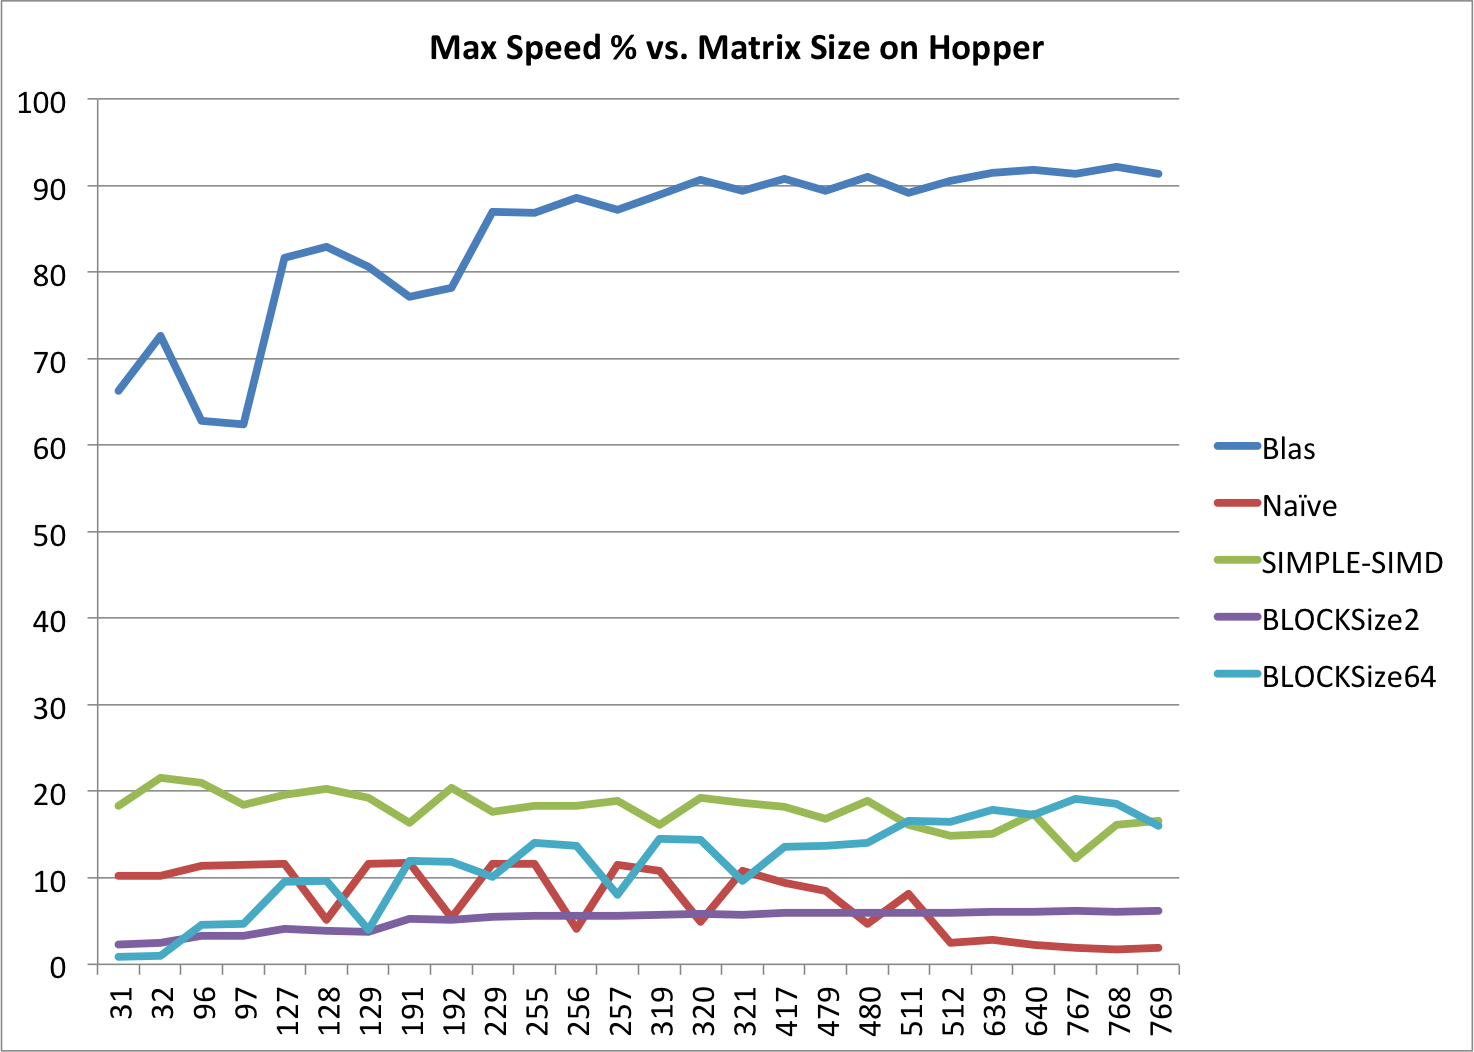
\includegraphics[width=\textwidth]{HopperChart1}
  \caption{Performance results on Hopper.}
  \label{fig:perf-hopper}
\end{figure}

We do see dips in performance for matrix sizes slightly above multiples of the block size.  As expected, this is most pronounced for the BLOCK algorithm with block size 64; the padding scheme means that a matrix of size 321 is padded to a matrix of size 384.

We also see that BLOCK begins to outperform SIMPLE-SIMD on large matrices.  Presumably this is due to cache locality.  The L1 cache of size 64KB on Hopper can hold 8,000 doubles, so when a matrix is larger than (roughly) 90-by-90, cache locality becomes relevant.  When SIMPLE-SIMD accesses a 16-by-16 block of a very large matrix, it loads 16*(cache line size) doubles into cache, only 256 of which are used.  The unused elements may be evicted from cache before the algorithm reaches them.  BLOCK wastes no loads in this way, since blocks are contiguous in memory.

\subsection{Performance on a laptop}
We also benchmarked our code on a mid-2013 Macbook Air with a 1.3GHz Intel Core i5 4250U.  Figure \ref{fig:perf-laptop} displays these performance results.  The results are qualitatively similar: BLOCK performs better and SIMPLE-SIMD performs worse as the matrix size increases.  But there is a huge utilization gap between the laptop and Hopper. For SIMPLE-SIMD, on our laptop the code can achieve a 50\% CPU utilization rate in average, while on Hopper it can only run at 16\%-18\% utilization on average.  Unfortunately, there are multiple differences between the laptop and a Hopper node.  The laptop has a much lower maximum CPU speed, but it also has an L1 cache size of 32KB, half of Hopper's 64KB.  So this test provides only weak evidence that the current bottleneck is in memory access.  We could test this hypothesis by implementing a fast version of MULTI, which would improve our memory access pattern over BLOCK.

\begin{figure}
  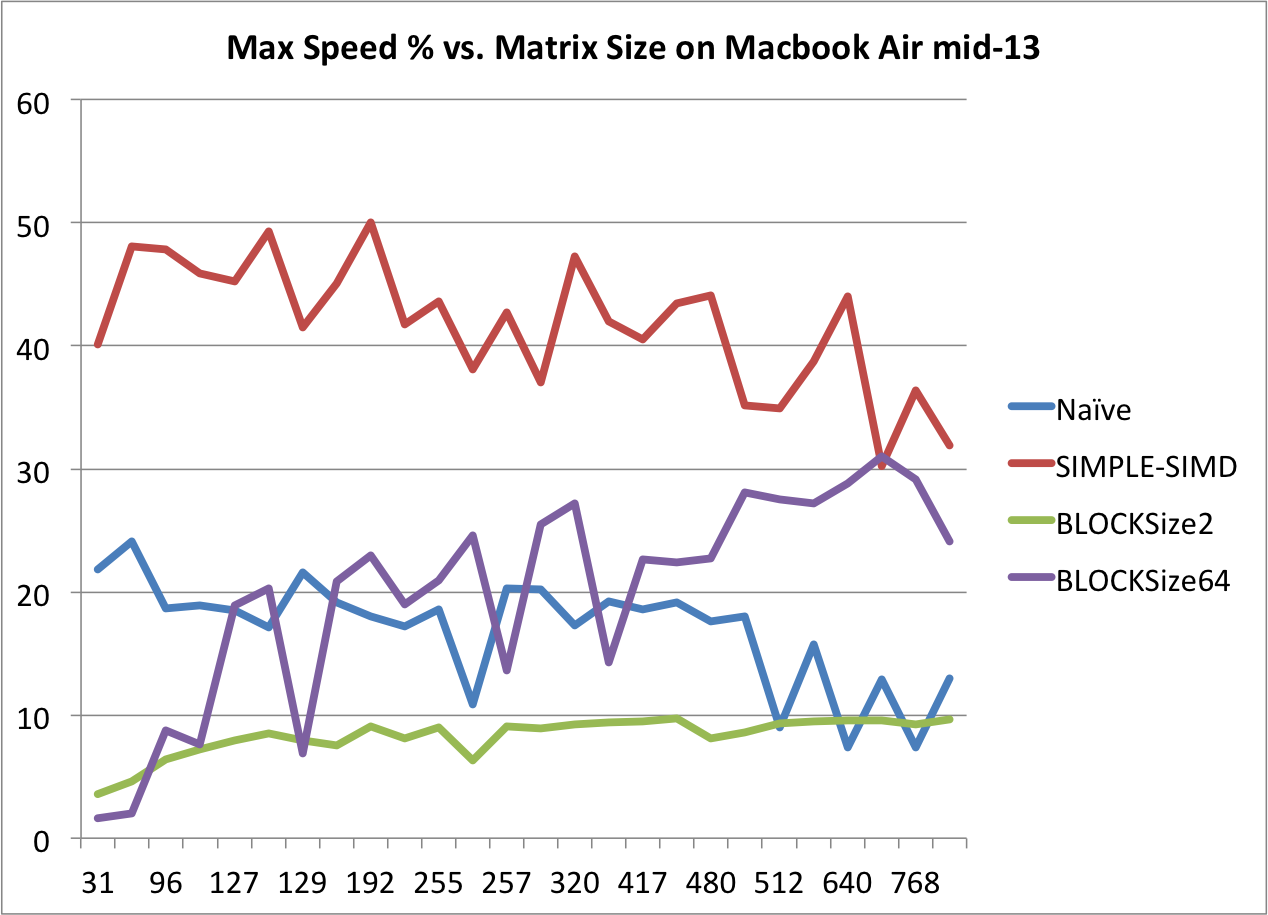
\includegraphics[width=\textwidth]{MacbookAirChart1}
  \caption{Performance results on a Macbook Air.}
  \label{fig:perf-laptop}
\end{figure}

\subsection{Copy overhead of BLOCK}
Finally, we investigated the cost of copying in the BLOCK algorithm.  To do this, we disabled the copy operation and ran the algorithm otherwise unchanged (which of course produces incorrect results).  Figure \ref{fig:copy-overhead} displays a comparison between this ``cheating'' version of BLOCK and the ordinary algorithm.  Copying seems to be responsible for the poor performance of BLOCK on small matrices, at least when the block size is 64.  (When the matrix size is 32 and the block size is 64, this figure reveals that BLOCK performs poorly for a different reason.  Likely that reason is that it performs 4 times as much computation as is necessary.)

\begin{figure}
  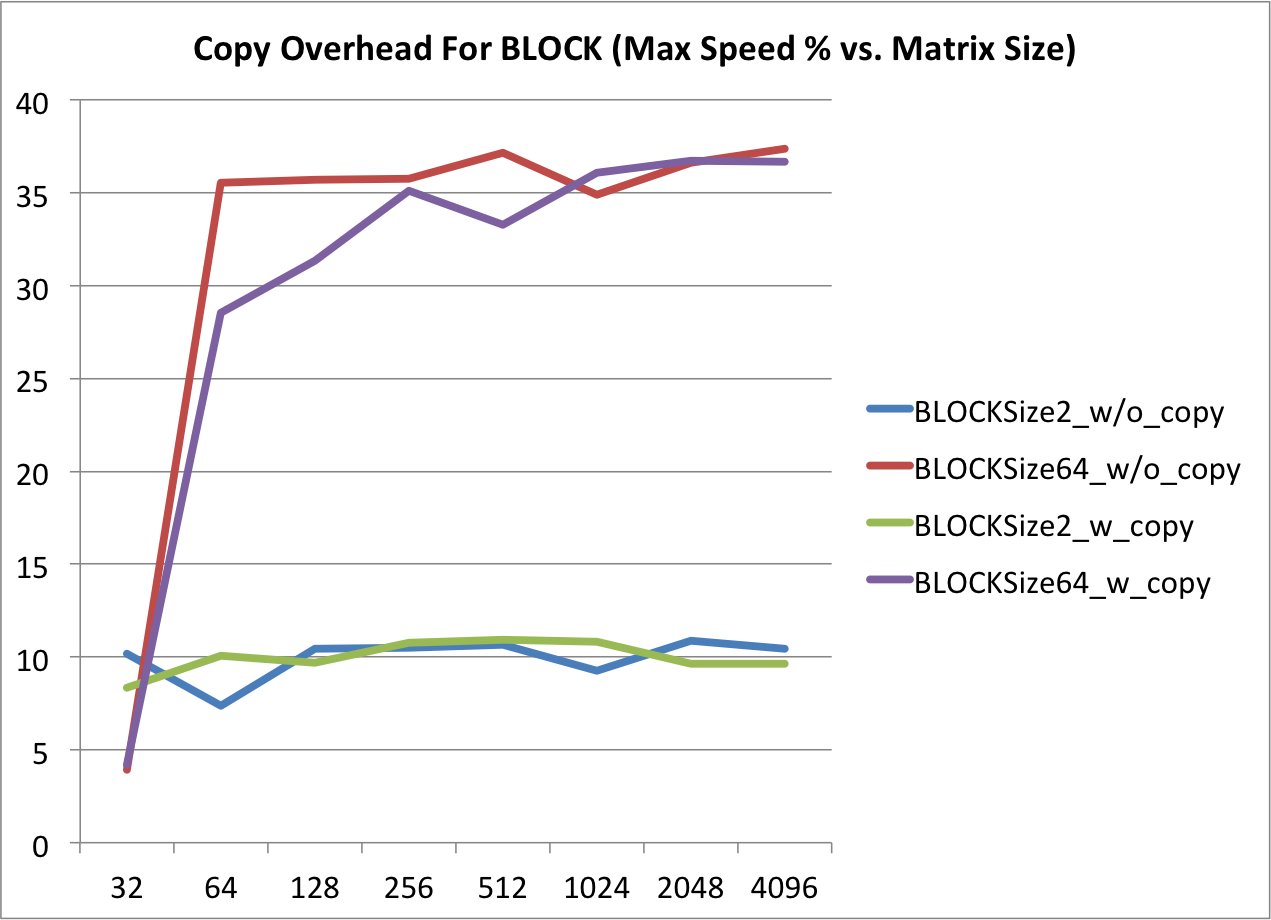
\includegraphics[width=\textwidth]{MacbookAirChart2}
  \caption{Performance results for the BLOCK algorithm with and without copy overhead.}
  \label{fig:copy-overhead}
\end{figure}

\end{document}